\documentclass{article}
\usepackage{amsmath, sfmath, multicol, tkz-euclide, array, enumerate, tcolorbox, tabularray}
\renewcommand{\familydefault}{\sfdefault}
\setlength{\parindent}{0cm}
\pagestyle{empty}
\usepackage[left=1in, top=0.5in, right=1in, bottom=0.5in]{geometry}
\tikzset{>=stealth}
\tcbset{colback=white}

\newcounter{example}[section]
\newenvironment{example}[1][]{\refstepcounter{example}\par\medskip
   {\color{red}\textbf{Example~\theexample. #1}}}{\medskip}

\begin{document}

\section*{Similar Solids}

\begin{tcolorbox}[colframe=orange!70!white, coltitle=black, title=\textbf{Today I Can}]
\begin{enumerate}
    \item Compare and find areas and volumes of similar solids
\end{enumerate}
\end{tcolorbox}
\smallskip

\begin{tcolorbox}[colframe=black!20!white, opacitybacktitle=0.1, coltitle=black, title=\textbf{Similar Solids}]
Solids that have the same shape and their corresponding dimensions are \emph{proportional}.
\end{tcolorbox}

\begin{example}
Determine whether each are similar.
\begin{multicols}{2}
\begin{enumerate}[(a)]
    \item \mbox{} \newline 
    \item \mbox{} \newline 
\end{enumerate}
\end{multicols}
\begin{minipage}{0.55\textwidth}
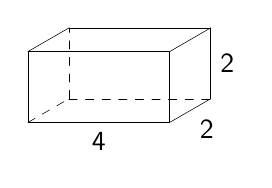
\begin{tikzpicture}[scale=0.6]
\tkzDefPoints{0/0/E, 3/0/F, 3/1.5/B, 0/1.5/A}
\tkzDrawPolygon(E,F,B,A)
\tkzDefShiftPoint[A](30:1){D}
\tkzDefShiftPoint[B](30:1){C}
\tkzDefShiftPoint[E](30:1){H}
\tkzDefShiftPoint[F](30:1){G}
\tkzDrawSegments(A,D B,C F,G D,C G,C)
\tkzDrawSegments[dashed](E,H H,D H,G)
% \tkzLabelPoints[left](A,E)
% \tkzLabelPoints[above left](D,H)
% \tkzLabelPoints[right](G,C)
% \tkzLabelPoints[right](B,F)
\tkzLabelSegment[below](E,F){4}
\tkzLabelSegment[below right](F,G){2}
\tkzLabelSegment[right](G,C){2}
\end{tikzpicture}
\hspace{0.25in}
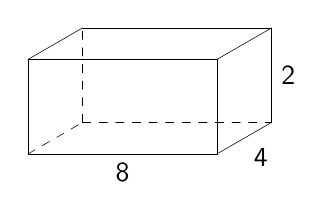
\begin{tikzpicture}[scale=0.8]
\tkzDefPoints{0/0/E, 3/0/F, 3/1.5/B, 0/1.5/A}
\tkzDrawPolygon(E,F,B,A)
\tkzDefShiftPoint[A](30:1){D}
\tkzDefShiftPoint[B](30:1){C}
\tkzDefShiftPoint[E](30:1){H}
\tkzDefShiftPoint[F](30:1){G}
\tkzDrawSegments(A,D B,C F,G D,C G,C)
\tkzDrawSegments[dashed](E,H H,D H,G)
% \tkzLabelPoints[left](A,E)
% \tkzLabelPoints[above left](D,H)
% \tkzLabelPoints[right](G,C)
% \tkzLabelPoints[right](B,F)
\tkzLabelSegment[below](E,F){8}
\tkzLabelSegment[below right](F,G){4}
\tkzLabelSegment[right](G,C){2}
\end{tikzpicture}
\end{minipage}
\begin{minipage}{0.43\textwidth}
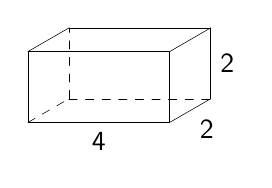
\begin{tikzpicture}[scale=0.6]
\tkzDefPoints{0/0/E, 3/0/F, 3/1.5/B, 0/1.5/A}
\tkzDrawPolygon(E,F,B,A)
\tkzDefShiftPoint[A](30:1){D}
\tkzDefShiftPoint[B](30:1){C}
\tkzDefShiftPoint[E](30:1){H}
\tkzDefShiftPoint[F](30:1){G}
\tkzDrawSegments(A,D B,C F,G D,C G,C)
\tkzDrawSegments[dashed](E,H H,D H,G)
% \tkzLabelPoints[left](A,E)
% \tkzLabelPoints[above left](D,H)
% \tkzLabelPoints[right](G,C)
% \tkzLabelPoints[right](B,F)
\tkzLabelSegment[below](E,F){4}
\tkzLabelSegment[below right](F,G){2}
\tkzLabelSegment[right](G,C){2}
\end{tikzpicture}
\hspace{0.25in}
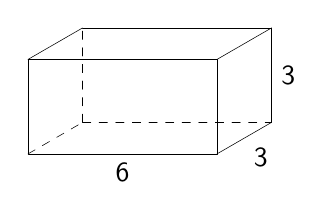
\begin{tikzpicture}[scale=0.8]
\tkzDefPoints{0/0/E, 3/0/F, 3/1.5/B, 0/1.5/A}
\tkzDrawPolygon(E,F,B,A)
\tkzDefShiftPoint[A](30:1){D}
\tkzDefShiftPoint[B](30:1){C}
\tkzDefShiftPoint[E](30:1){H}
\tkzDefShiftPoint[F](30:1){G}
\tkzDrawSegments(A,D B,C F,G D,C G,C)
\tkzDrawSegments[dashed](E,H H,D H,G)
% \tkzLabelPoints[left](A,E)
% \tkzLabelPoints[above left](D,H)
% \tkzLabelPoints[right](G,C)
% \tkzLabelPoints[right](B,F)
\tkzLabelSegment[below](E,F){6}
\tkzLabelSegment[below right](F,G){3}
\tkzLabelSegment[right](G,C){3}
\end{tikzpicture}
\end{minipage}
\end{example}

\vspace{0.5in}

\begin{tcolorbox}[colframe=black!20!white, opacitybacktitle=0.1, coltitle=black, title=\textbf{Areas and Volumes of Similar Solids}]
If the scale factor of two similar solids is $a \, : \, b$

\begin{multicols}{2}
\begin{itemize}
    \item Surface Areas
    \begin{itemize}
        \item $a^2 \, : \, b^2$
        \item (scale factor)$^2$
    \end{itemize}
    \item Volumes
    \begin{itemize}
        \item $a^3 \, : \, b^3$
        \item (scale factor)$^3$
    \end{itemize}
\end{itemize}
\end{multicols}
\end{tcolorbox}

\bigskip 

\begin{example}
Find the ratios of surface areas and ratios of volumes for each.  
\begin{multicols}{2}
\begin{enumerate}[(a)]
    \item \mbox{} \newline 
    \item \mbox{} \newline 
\end{enumerate}
\end{multicols}
\begin{minipage}{0.5\textwidth}
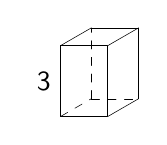
\begin{tikzpicture}[scale=0.6]
\tkzDefPoints{0/0/A, 1/0/B, 1/1.5/C, 0/1.5/D}
\tkzDefShiftPoint[A](30:0.75){E}
\tkzDefShiftPoint[B](30:0.75){F}
\tkzDefShiftPoint[C](30:0.75){G}
\tkzDefShiftPoint[D](30:0.75){H}
\tkzDrawPolygon(A,B,C,D)
\tkzDrawSegments[dashed](A,E E,H E,F)
\tkzDrawSegments(B,F C,G D,H H,G G,F)
\tkzLabelSegment[left](A,D){3}
\end{tikzpicture}
\hspace{0.25in}
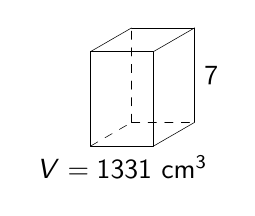
\begin{tikzpicture}[scale=0.8]
\tkzDefPoints{0/0/A, 1/0/B, 1/1.5/C, 0/1.5/D}
\tkzDefShiftPoint[A](30:0.75){E}
\tkzDefShiftPoint[B](30:0.75){F}
\tkzDefShiftPoint[C](30:0.75){G}
\tkzDefShiftPoint[D](30:0.75){H}
\tkzDrawPolygon(A,B,C,D)
\tkzDrawSegments[dashed](A,E E,H E,F)
\tkzDrawSegments(B,F C,G D,H H,G G,F)
\tkzLabelSegment[right](F,G){7}
\tkzLabelSegment[below](A,B){$V=1331$ cm$^3$}
\end{tikzpicture}
\end{minipage}
\begin{minipage}{0.4\textwidth}
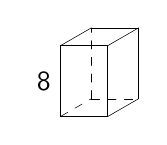
\begin{tikzpicture}[scale=0.6]
\tkzDefPoints{0/0/A, 1/0/B, 1/1.5/C, 0/1.5/D}
\tkzDefShiftPoint[A](30:0.75){E}
\tkzDefShiftPoint[B](30:0.75){F}
\tkzDefShiftPoint[C](30:0.75){G}
\tkzDefShiftPoint[D](30:0.75){H}
\tkzDrawPolygon(A,B,C,D)
\tkzDrawSegments[dashed](A,E E,H E,F)
\tkzDrawSegments(B,F C,G D,H H,G G,F)
\tkzLabelSegment[left](A,D){8}
\end{tikzpicture}
\hspace{0.25in}
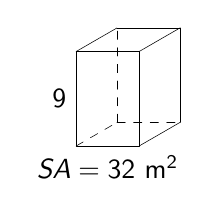
\begin{tikzpicture}[scale=0.8]
\tkzDefPoints{0/0/A, 1/0/B, 1/1.5/C, 0/1.5/D}
\tkzDefShiftPoint[A](30:0.75){E}
\tkzDefShiftPoint[B](30:0.75){F}
\tkzDefShiftPoint[C](30:0.75){G}
\tkzDefShiftPoint[D](30:0.75){H}
\tkzDrawPolygon(A,B,C,D)
\tkzDrawSegments[dashed](A,E E,H E,F)
\tkzDrawSegments(B,F C,G D,H H,G G,F)
\tkzLabelSegment[left](A,D){9}
\tkzLabelSegment[below](A,B){$SA=32$ m$^2$}
\end{tikzpicture}
\end{minipage}
\end{example}

\newpage 

\begin{example}
The solid is similar to a larger solid with the given scale factor.
\newline

Find the surface area and volume of the larger solid.
\newline

Scale Factor = 1 : 4
\newline

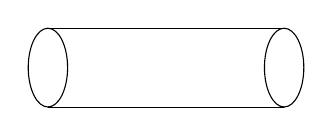
\begin{tikzpicture}
\tkzDefPoints{0/0/A, 3/0/B, 0/-1/D, 3/-1/C}
\tkzDrawSegments(A,B C,D)
\draw (0,-0.5) ellipse (0.25 and 0.5);
\draw (3,-0.5) ellipse (0.25 and 0.5);
\end{tikzpicture}
\end{example}


\end{document}
